\chapter{
شمای پایگاه داده
}

در این فصل شمای
\footnote{\lr{schema}}
 پایگاه داده مشخص شده است. در هر جدول نوع مقدار، کلیدهای اصلی، کلیدهای خارجی، قابل تهی
\footnote{\lr{Null}}
 بودن مقدار و همچنین متمایز
 \footnote{\lr{Unique}}
  بودن آن مشخص شده است.
\begin{figure}[h]
	\centering
	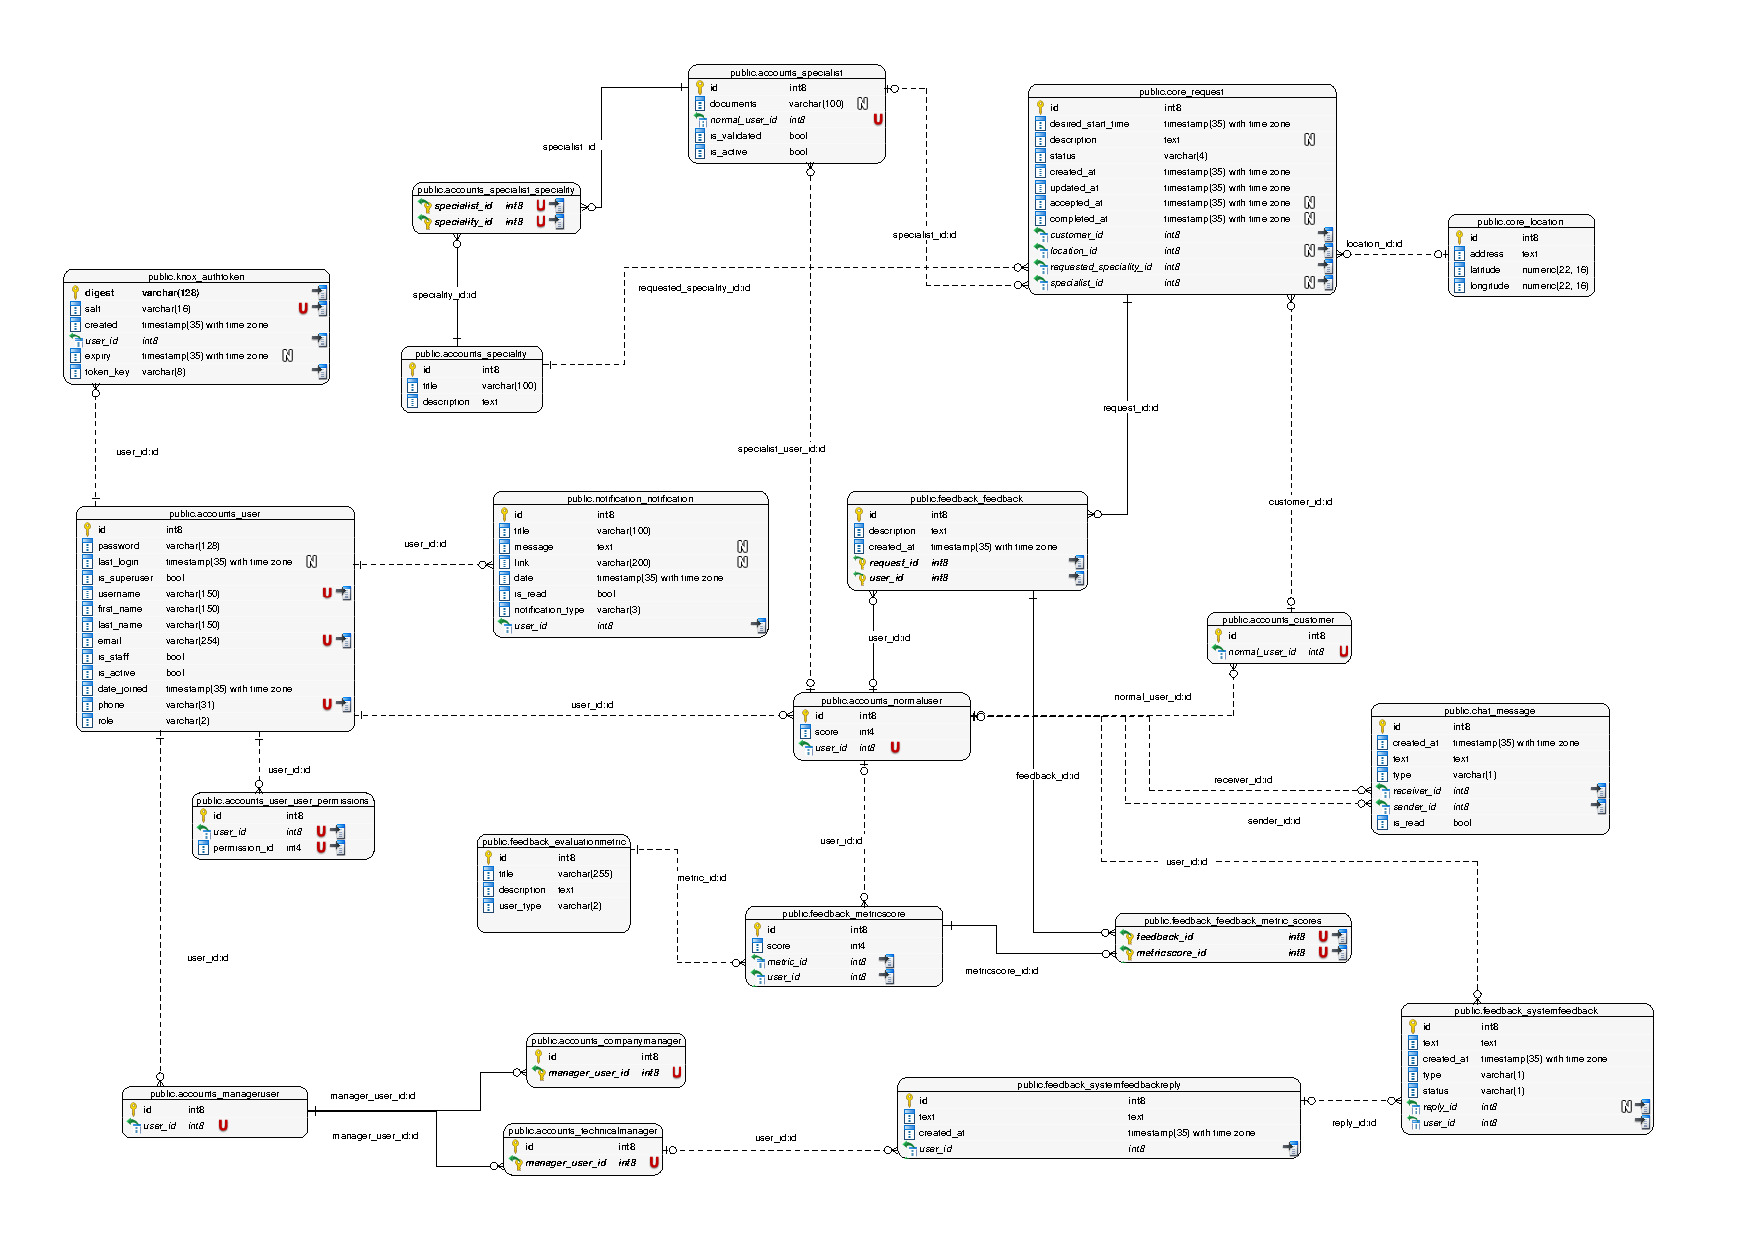
\includegraphics[width=\textwidth]{figs/entity-relationship}
	\caption{شمای پایگاه داده}
	\label{database-schema}
\end{figure}

